
\chapter{Numerical Validation}
\label{chp:NumMethodComp}
In this chapter analytic and forced solutions are used to validate the numerical methods. 

%Analytic comparions
%Forced solutions

To verify that the numerical methods have the expected convergence and conservation properties we make use of the analytic and forced solutions described in Chapter \ref{chp:Serreeqns}. To assess these properties we first introduce the measures of convergence and conservation for a numerical solution. These measures are then used to compare all the numerical methods using the solitary travelling wave solution. The convergence and conservation properties of $\text{FDVM}_2$ and $\text{FEVM}_2$ are compared using the lake at rest solution. Currently, the $\text{FDVM}_2$ and $\text{FEVM}_2$ are the only methods in this thesis that incorporate varying bathymetry.

Finally we validate $\text{FDVM}_2$ and $\text{FEVM}_2$ using forced solutions which test the accuracy of their approximations to all terms in the Serre equations. The forced solutions are obtained by adding terms to the Serre equations \eqref{eqn:FullSerreConForced} to force any desired solution. This allows the method to be validated against more flow scenarios than possible given the limited number of currently known analytic solutions. These forced solutions can be any functions and so the forced Serre equations are no longer strictly conservative. Therefore, the forced solutions are only used to assess the convergence properties of these numerical methods. 

\section{Measuring Convergence and Conservation}
The convergence of the numerical methods is studied by comparing their numerical solutions to the analytic solutions or the forced solutions of the Serre equations. While conservation is investigated by comparing the total amount of a conserved quantity in a numerical solution at some time with the total amount of that quantity present in the initial conditions. We introduce notation for these measures and describe their calculation here, beginning with convergence.

\subsection{Measure of Convergence}
By measuring the relative difference between the numerical and analytic solutions as $\Delta x$ varies, the convergence of the numerical methods can be investigated. To measure the relative difference we use the $L_2$ vector norm; to compare the numerical and analytic solutions at the cell midpoints $x_j$ at the end of the simulations. For a quantity $q$, the vector of its values $\vecn{q}$ at the cell midpoints $x_j$ and the corresponding numerical solution at those locations $\vecn{q^*}$; the $L_2$ norm is
\begin{equation*}
L_2(\vecn{q},\vecn{q^*}) =  \left\lbrace \begin{array}{c r} 
\dfrac{||\vecn{q^*} - \vecn{q}||_{2}}{||\vecn{q}||_{2}} & ||\vecn{q}||_{2} > 0 \\ \\
{||\vecn{q^*}||_{2}} & ||\vecn{q}||_{2} = 0 . \end{array}\right. 
\label{eqn:L1qdef} 
\end{equation*}


%When no analytic solution is present, we can compare the distance between numerical solutions to gain some insight into how a sequence of numerical solutions are behaving. This allows us to demonstrate that a sequence of numerical solutions is convergent to some solution. To do this the $L_1$ vector norm is again used as in \eqref{eqn:L1qdef} except now both vectors are numerical solutions. Since both numerical solutions will have different grid locations, we only take the difference between the two at the common grid points. We have constructed our grids to accommodate for this, varying $\Delta x$ by successively dividing by $2$. This ensures that the grid locations generated by the larger $\Delta x$ value are all in the grid generated by the smaller $\Delta x$ value, and so we can compare both numerical solutions at the grid points generated by the larger $\Delta x$ value.  


\subsection{Measures of Conservation}
The conservation properties of the methods are established by calculating the total amount of a conserved quantity in the numerical solution $\mathcal{C}^*\left({\vecn{q^*}}\right)$ at the end of the simulation and comparing it to the total amount of that quantity present in the initial conditions $\mathcal{C}\left({q(x,0)} \right)$, derived analytically. Again a relative measure is used;
\begin{equation}
C(q,\vecn{q^*}) =  \left\lbrace \begin{array}{c r} 
\dfrac{|\mathcal{C}^*\left({\vecn{q^*}}\right) - \mathcal{C}\left({q(x,0)} \right)| }{|\mathcal{C}\left({q(x,0)} \right)|} & |\mathcal{C}\left({q(x,0)} \right)| > 0 \\ \\
|\mathcal{C}^*\left({\vecn{q^*}}\right)| & |\mathcal{C}\left({q(x,0)} \right)| = 0  \end{array}\right. 
\label{eqn:C1qdef} 
\end{equation}
where $\mathcal{C}^*\left({\vecn{q^*}}\right)$ was calculated using 3 point Gaussian quadrature over the $j^{th}$ cell and summing these cell integrals for all $j$. The value of $q$ at the three points needed to perform the Gaussian quadrature were calculated by interpolating the $j^{th}$ cell using a quartic polynomial that fits the nodal values $q_{j-2}$, $q_{j-1}$, $q_{j}$, $q_{j+1}$ and $q_{j+2}$ at the surrounding cell midpoints. Gaussian quadrature using three points is $5^{th}$ order accurate and interpolation by quartics is $5^{th}$ order accurate for the quantity $q$ and $4^{th}$ order accurate for its spatial derivative $\partial q /  \partial x$. Since all methods are third-order accurate or less, the error introduced by the calculation of $\mathcal{C}^*\left({\vecn{q^*}}\right)$ for $h$, $uh$, $G$ and $\mathcal{H}$ will be dominated by the error introduced by the numerical solvers.

In some cases $\mathcal{C}\left({q(x,0)} \right)$ may be difficult to derive analytically. In this case we approximate $\mathcal{C}\left({q(x,0)} \right)$ with $\mathcal{C}^*\left(\vecn{q}^0\right)$ in \eqref{eqn:C1qdef}; where $\vecn{q}^0$ is the vector of the quantity at the cell midpoints used as the initial conditions of our numerical method. We denote the numerical approximation to the conservation error \eqref{eqn:C1qdef} by $C^*$. This conservation error will also be more enlightening in cases where the errors introduced by the discretisation are large, as these errors will be similar for $\mathcal{C}^*\left(\vecn{q}^0\right)$ and $\mathcal{C}^*\left(\vecn{q^*}\right)$. 


\section{Solitary Travelling Wave Solution}
%Maybe a bit of description about what it lookds like?
To assess the ability of our numerical methods to solve the Serre equations with a horizontal bed we use the solitary travelling wave solution \eqref{eqn:Solitondefhub} described in Chapter \ref{chp:Serreeqns}. This is a particular member of the family of periodic travelling wave solutions \cite{El-etal-2006}. Every member of this family of solutions except the trivial stationary one have the same non-zero terms and thus provide similar tests for the numerical methods. Hence, it is sufficient to only study the solitary travelling wave solution.

For the solitary wave solution all the terms in \eqref{eqn:FullSerreConHorizBed} must be adequately approximated by the numerical method to properly reproduce the analytic solution. Therefore, this analytic solution serves as a benchmark for the ability of a numerical method to accurately solve the Serre equations with a horizontal bed for smooth solutions.

For our numerical tests we used the solitary travelling wave solution \eqref{eqn:Solitondefhub} with $a_0 = 1m$ , $a_1 = 0.7m$ and $g= 9.81m/s^2$ at $t=0s$ as the initial conditions. The spatial domain was $[-250m,250m]$ and the problem was solved until $t= 50s$. This was done for a range of $\Delta x$ values that had the following form; $\Delta x = 100 / 2^k m$ with $k \in  \left[6,\dots,19\right]$. The CFL condition was satisfied with CFL number $Cr = 0.5$ by setting $\Delta t = Cr \Delta x / \sqrt{g\left(a_0 + a_1\right)}$. For $\text{FDVM}_2$ and $\text{FEVM}_2$ the limiting parameter $\theta  = 1.2$ was used in the generalised minmod limiter \eqref{eqn:slopehGrecon} employed by both methods during the reconstruction step. While $\text{FDVM}_3$ used a Koren limiter in its reconstruction \cite{Zoppou-etal-2017}, which has no limiting parameter. 

For the parameters $a_0 = 1m$ and $a_1 = 0.7m$ the non-linearity is $\epsilon = a_1 / a_0 = 0.7$; this is large but beneath most of the well known breaking thresholds for water waves $\epsilon \le 0.8$ \cite{Ippen-Kulin-1954-4}. Because $\epsilon$ is large the non-linear effects are large and therefore, so are the balancing dispersive effects making this particular analytic solution a rigorous test of the numerical methods. For this spatial domain and final time $t=50s$ there is no interaction of the wave with the boundary, therefore the Dirichlet boundary conditions were appropriate.

The results of this analytic solution validation were published by \citet{Zoppou-etal-2017} for $\text{FDVM}_1$, $\text{FDVM}_2$ and $\text{FDVM}_3$. I produced the results in that paper which have been expanded here to include an investigation of the convergence of $G$ and the conservation of $h$, $uh$ and $G$.

An example numerical solution with $\Delta x = {100} / {2^{11}}m \approx 0.049m$ from all methods was plotted in Figure \ref{fig:SolitonExAll} against the analytic solution at $t= 50s$. We have only plotted an illustrative amount of the points in the numerical solution. From these plots it is clear that $\text{FDVM}_1$ performs significantly worse than the high-order methods at reproducing the analytic solution, even for this relatively fine grid where the wave is captured by more than $200$ cells. This is primarily due to the numerical diffusion introduced by the method, which has caused the wave in the numerical solution to decrease in amplitude and widen significantly. The high-order numerical methods all accurately replicate the analytic solution, with insignificant visual differences in these plots due to the high resolution of the grid.

\begin{figure}
	\centering
	\begin{subfigure}{0.5\textwidth}
		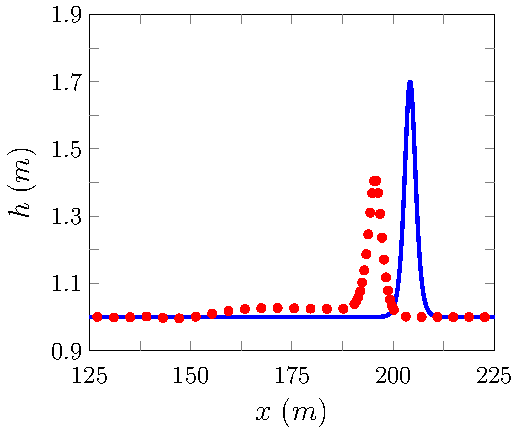
\includegraphics[width=\textwidth]{./chp5/figures/Analytic/Soliton/Example/FDVM1.pdf}
		\subcaption{$\text{FDVM}_1$}
		\vspace{0.5cm}
	\end{subfigure}%
	\begin{subfigure}{0.5\textwidth}
		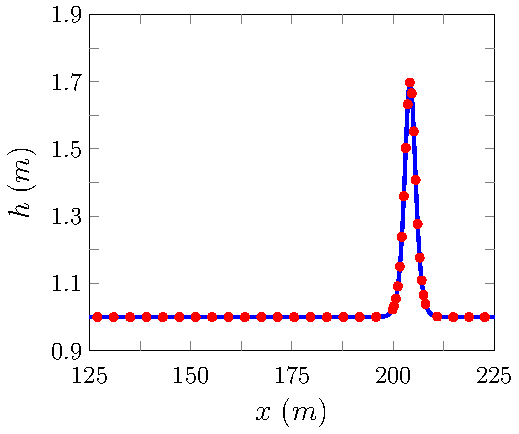
\includegraphics[width=\textwidth]{./chp5/figures/Analytic/Soliton/Example/FDVM2.pdf}
		\subcaption{$\text{FDVM}_2$}
		\vspace{0.5cm}
	\end{subfigure}
	\begin{subfigure}{0.5\textwidth}
		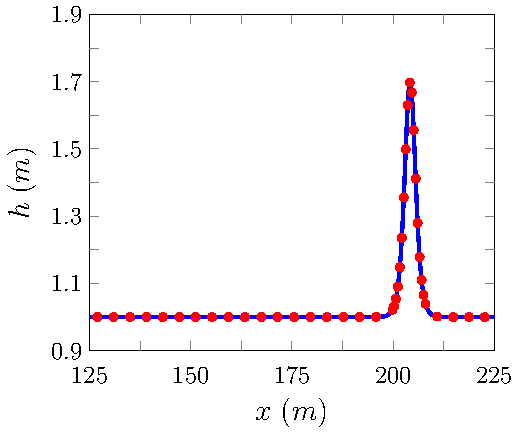
\includegraphics[width=\textwidth]{./chp5/figures/Analytic/Soliton/Example/FEVM2.pdf}
		\subcaption{$\text{FEVM}_2$}
		\vspace{0.5cm}
	\end{subfigure}%
	\begin{subfigure}{0.5\textwidth}
		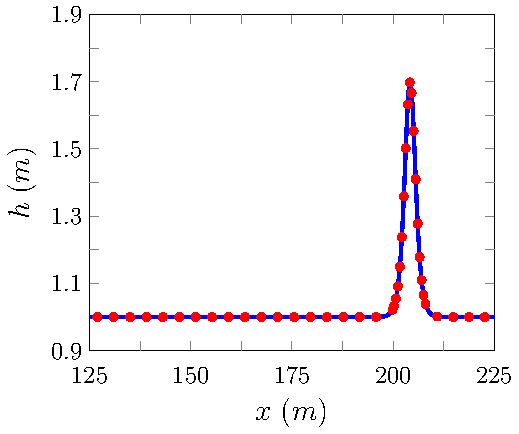
\includegraphics[width=\textwidth]{./chp5/figures/Analytic/Soliton/Example/FDVM3.pdf}
		\subcaption{$\text{FDVM}_3$}
		\vspace{0.5cm}
	\end{subfigure}
	\begin{subfigure}{0.5\textwidth}
		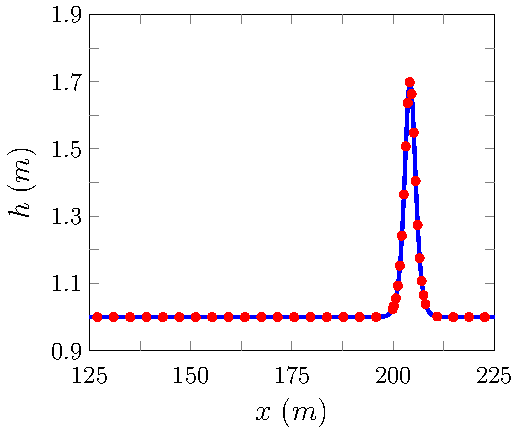
\includegraphics[width=\textwidth]{./chp5/figures/Analytic/Soliton/Example/D.pdf}
		\subcaption{$\mathcal{D}$}
	\end{subfigure}%
	\begin{subfigure}{0.5\textwidth}
		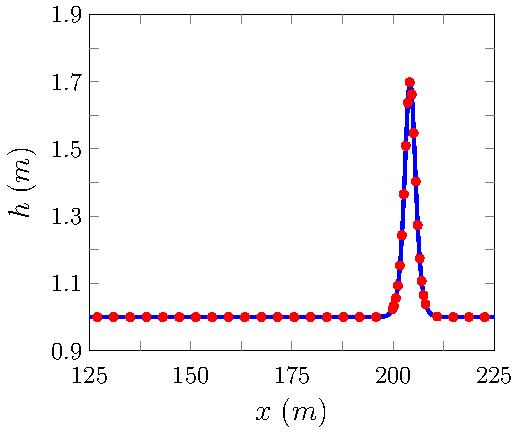
\includegraphics[width=\textwidth]{./chp5/figures/Analytic/Soliton/Example/W.pdf}
		\subcaption{$\mathcal{W}$}
	\end{subfigure}
	\caption{Comparison of the analytic solution ({\color{blue} \solidrule}) and numerical solution with $\Delta x = {100} / {2^{11}}m$ ({\color{red} $\bullet$}) for the solitary travelling wave solution at $t=50s$ for all methods.}
	\label{fig:SolitonExAll}
\end{figure}


The $L_2$ error was calculated for $h$, $u$ and $G$ for all numerical solutions and was plotted against $\Delta x$ for all numerical methods in Figure \ref{fig:SolitonL1All}. From these plots it is clear that all numerical methods are convergent. The rate at which the numerical solutions converge to the analytic solution over $\Delta x$ is determined by the order of accuracy of the numerical scheme. All methods demonstrate the expected order of accuracy given the order of accuracy of the approximations used in the method; which agrees with the results of the linear analysis in Chapter \ref{chp:AnalNumMethod} and Appendix \ref{app:LinAnal}. 
\begin{figure}
	\centering
	\begin{subfigure}{0.5\textwidth}
		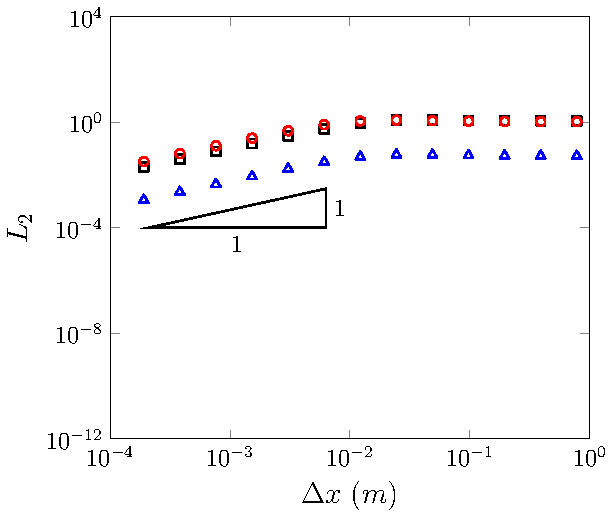
\includegraphics[width=\textwidth]{./chp5/figures/Analytic/Soliton/L2/FDVM1.pdf}
		\subcaption{$\text{FDVM}_1$}
		\vspace{0.5cm}
	\end{subfigure}%
	\begin{subfigure}{0.5\textwidth}
		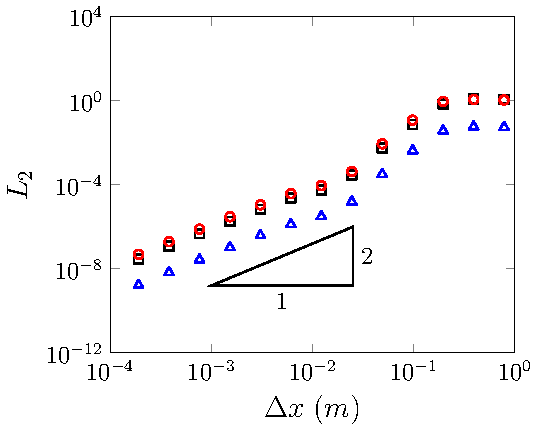
\includegraphics[width=\textwidth]{./chp5/figures/Analytic/Soliton/L2/FDVM2.pdf}
		\subcaption{$\text{FDVM}_2$}
		\vspace{0.5cm}
	\end{subfigure}
	\begin{subfigure}{0.5\textwidth}
		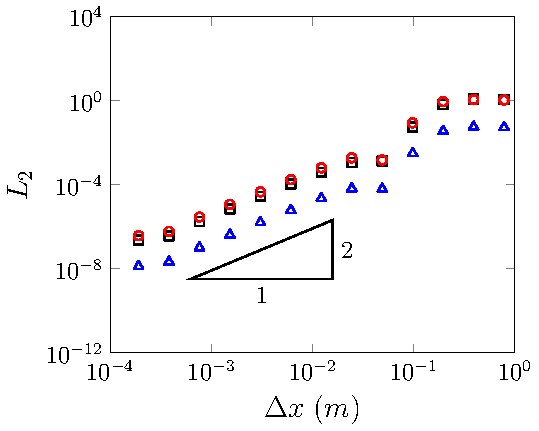
\includegraphics[width=\textwidth]{./chp5/figures/Analytic/Soliton/L2/FEVM2.pdf}
		\subcaption{$\text{FEVM}_2$}
		\vspace{0.5cm}
	\end{subfigure}%
	\begin{subfigure}{0.5\textwidth}
		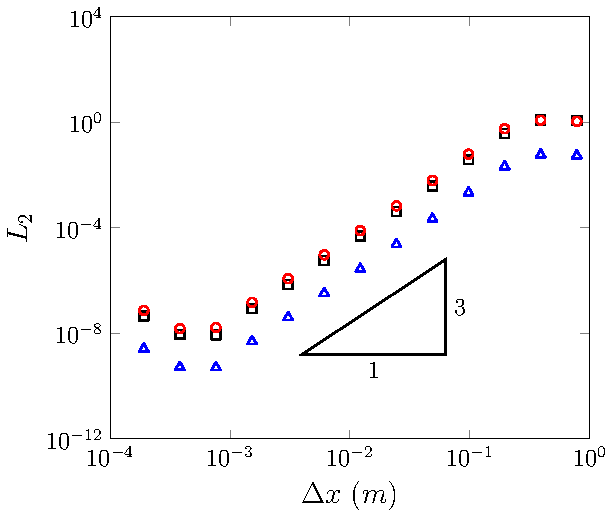
\includegraphics[width=\textwidth]{./chp5/figures/Analytic/Soliton/L2/FDVM3.pdf}
		\subcaption{$\text{FDVM}_3$}
		\vspace{0.5cm}
	\end{subfigure}
	\begin{subfigure}{0.5\textwidth}
		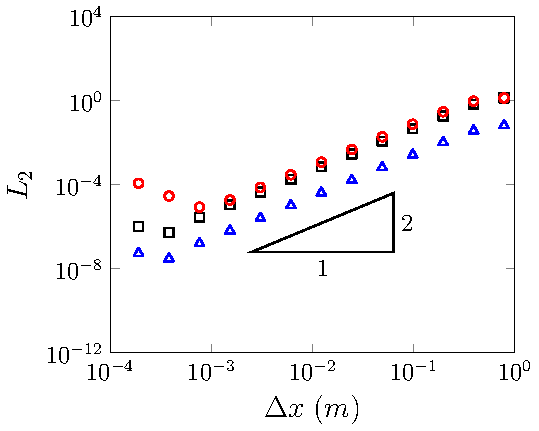
\includegraphics[width=\textwidth]{./chp5/figures/Analytic/Soliton/L2/D.pdf}
		\subcaption{$\mathcal{D}$}
	\end{subfigure}%
	\begin{subfigure}{0.5\textwidth}
		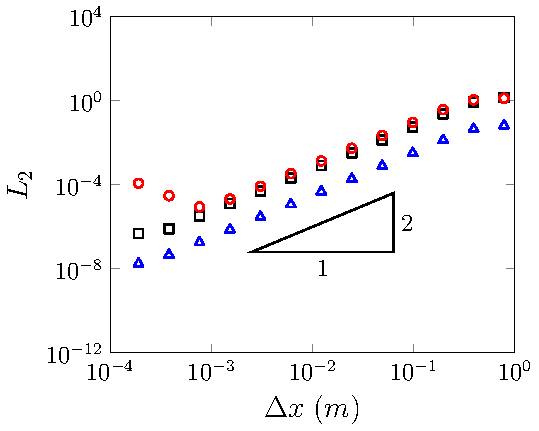
\includegraphics[width=\textwidth]{./chp5/figures/Analytic/Soliton/L2/W.pdf}
		\subcaption{$\mathcal{W}$}
	\end{subfigure}
	\caption{Convergence as measured by the $L_2$ norm against $\Delta x$ for $h$ (\trianglet{blue}), $u$ (\squaret{black}) and $G$ (\circlet{red}) for the soliton problem for all methods.}
	\label{fig:SolitonL1All}
\end{figure}

All methods more accurately reproduced the analytic solution for $h$ than either $G$ or $u$ across all $\Delta x$ values. This is due to the simplicity of $h$'s evolution equation \eqref{eqn:FullSerreConMass} compared to the evolution equation of $G$ \eqref{eqn:Serreconsconmom}; with the error in $u$ being dominated by the error in $G$. 

Increasing the order of accuracy of our numerical methods leads to smaller errors when comparing two numerical solutions for the same $\Delta x$ value, as Figure \ref{fig:SolitonL1All} clearly demonstrates. This is consistent with the example numerical solution in Figure \ref{fig:SolitonExAll}, where the lowest order accuracy scheme, $\text{FDVM}_1$ had the poorest reproduction of the analytic solution. However, there is only a slight benefit from moving from the second-order $\text{FEVM}_2$ and $\text{FDVM}_2$ to the third-order $\text{FDVM}_3$.

For the second-order methods we find that $\text{FDVM}_2$ consistently produces the smallest $L_2$ error followed by $\text{FEVM}_2$, $\mathcal{W}$ and $\mathcal{D}$. The difference between the $\text{FDVM}_2$ and $\text{FEVM}_2$ is significant with the errors of $\text{FEVM}_2$ being $2$ to $4$ times larger than those of $\text{FDVM}_2$. Therefore, $\text{FDVM}_2$ is reproducing the solitary wave solution more accurately than $\text{FEVM}_2$.

The finite difference methods produce very similar errors which are twice as large as the errors from $\text{FEVM}_2$. Additionally, the round-off effects dominate the $L_2$ error of the finite difference methods at larger $\Delta x$ values than for the finite volume based methods.

The error in conservation $C$ was calculated for all methods using the analytic expressions for the total amounts of the conserved quantities in the initial conditions \eqref{eqn:SolitonConservation}. The error in conservation was plotted against the spatial resolution in Figure \ref{fig:SolitonC1All}. These results demonstrate that due to the use of the finite volume methods for $h$ and $G$, both are conserved at round-off error for all the finite volume based methods as expected. While the finite difference methods only conserved $h$ at round-off error because the employed finite difference method for the continuity equation \eqref{eqn:FullSerreConMass} is a conservative method. 

\begin{figure}
	\centering
	\begin{subfigure}{0.5\textwidth}
		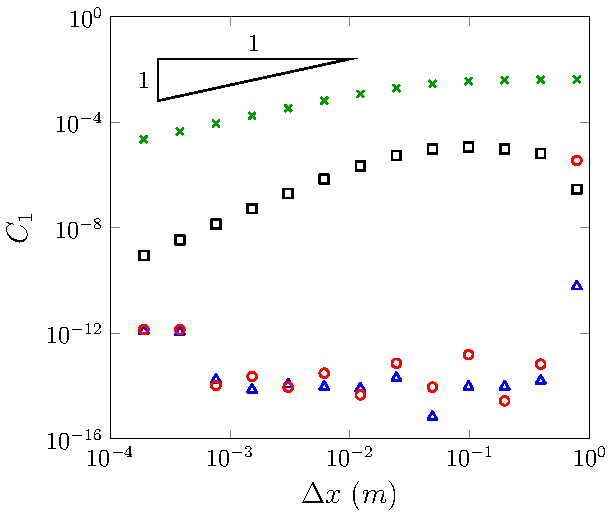
\includegraphics[width=\textwidth]{./chp5/figures/Analytic/Soliton/C1/FDVM1.pdf}
		\subcaption{$\text{FDVM}_1$}
		\vspace{0.3cm}
	\end{subfigure}%
	\begin{subfigure}{0.5\textwidth}
		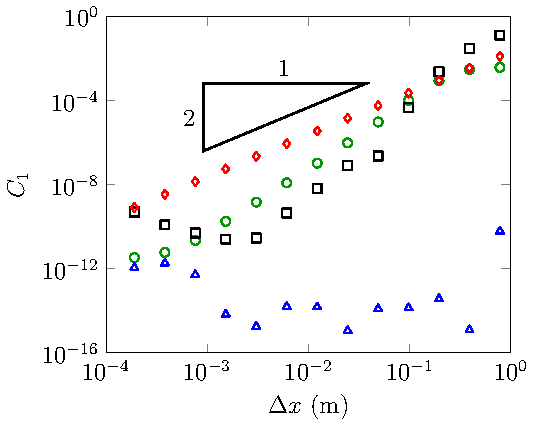
\includegraphics[width=\textwidth]{./chp5/figures/Analytic/Soliton/C1/FDVM2.pdf}
		\subcaption{$\text{FDVM}_2$}
		\vspace{0.3cm}
	\end{subfigure}
	\begin{subfigure}{0.5\textwidth}
		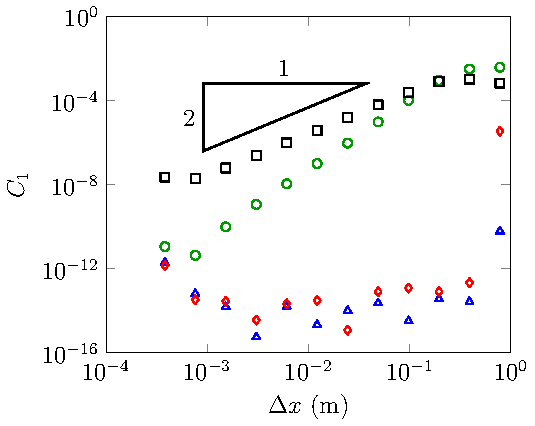
\includegraphics[width=\textwidth]{./chp5/figures/Analytic/Soliton/C1/FEVM2.pdf}
		\subcaption{$\text{FEVM}_2$}
		\vspace{0.3cm}
	\end{subfigure}%
	\begin{subfigure}{0.5\textwidth}
		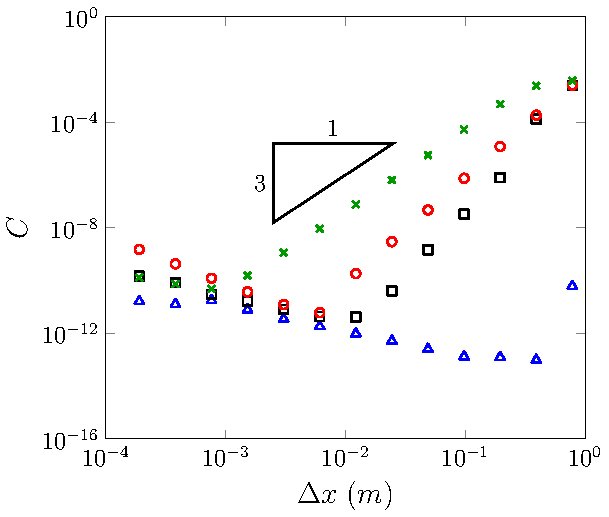
\includegraphics[width=\textwidth]{./chp5/figures/Analytic/Soliton/C1/FDVM3.pdf}
		\subcaption{$\text{FDVM}_3$}
		\vspace{0.3cm}
	\end{subfigure}
	\begin{subfigure}{0.5\textwidth}
		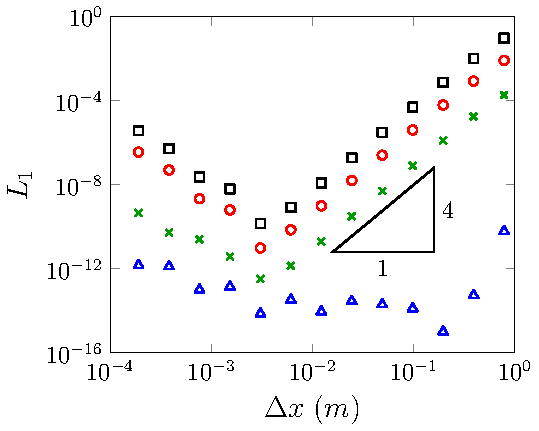
\includegraphics[width=\textwidth]{./chp5/figures/Analytic/Soliton/C1/D.pdf}
		\subcaption{$\mathcal{D}$}
	\end{subfigure}%
	\begin{subfigure}{0.5\textwidth}
		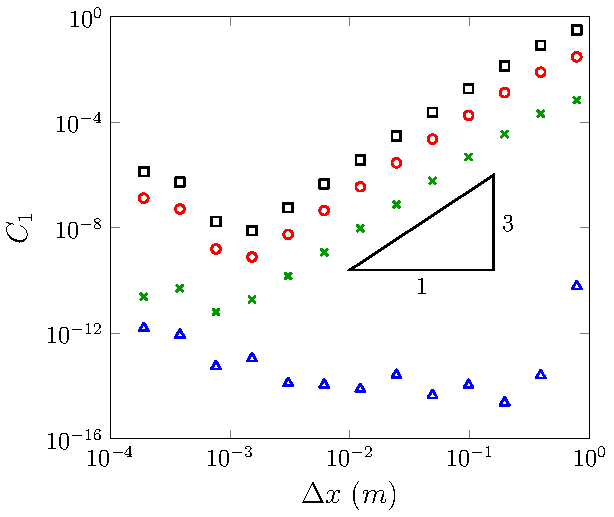
\includegraphics[width=\textwidth]{./chp5/figures/Analytic/Soliton/C1/W.pdf}
		\subcaption{$\mathcal{W}$}
	\end{subfigure}
	\caption{Conservation error $C$ against $\Delta x$ for $h$ (\trianglet{blue}), $uh$ (\squaret{black}), $G$ (\circlet{red}) and $\mathcal{H}$ ({\crosst{green!60!black}}) for the solitary travelling wave solution for all methods.}
	\label{fig:SolitonC1All}
\end{figure}

No methods conserve $\mathcal{H}$ or the $uh$ within machine precision. Since none of the methods were designed to conserve these quantities this is not surprising, although the error in conservation of all methods for these quantities does exhibit the order of accuracy of the convergence of the numerical method or better, as expected. 

For small $\Delta x$ values the round-off errors dominate the conservation error, particularly for the finite difference methods. Interestingly, $\text{FDVM}_3$ has an accumulation of round-off error increasing the conservation error for $h$ and $G$ as $\Delta x$ decreases. This was found to be caused by the Runge-Kutta coefficients of the third-order time stepping method \cite{Zoppou-etal-2017} not being exactly represented as floating point numbers. For the third-order SSP Runge-Kutta time stepping method the coefficients in the last step are $1/3$ and $2/3$. Since these numbers are not exactly represented in floating point they are approximated with a small error that when summed does not maintain the conservation properties of $h$ and $G$. Thus, every time step accumulates a small conservation error of machine precision size leading to the observed increase as $\Delta x$ becomes small and the number of time steps increases. Remedies for this were attempted such as using the coefficients $1/3$ and $(1- 1/3)$ and bringing the common divisor out but this problem persisted. Some other numerical techniques are required to resolve this issue such as those of \citet{higham2002}. Ultimately, since the convergence of $\text{FDVM}_3$ was only slightly better than $\text{FEVM}_2$ and $\text{FDVM}_2$ \cite{Zoppou-etal-2017} it was not developed further and this issue was not resolved.

These results demonstrate the need for high-order accurate schemes to accurately approximate the Serre equations. Furthermore, they suggest that second-order accuracy is sufficient, with third-order accurate schemes showing only a slight improvement. This was also the conclusion of the analytic validation by \citet{Zoppou-etal-2017}. Finally, they demonstrate the ability of FEVM and FDVM to conserve $h$ and $G$ up to machine precision, as desired. Given these results, only $\text{FEVM}_2$ and $\text{FDVM}_2$ have been extended to allow for variable bathymetry and dry beds. Consequently, the rest of the results in this chapter and Chapter \ref{chp:ExpMethodComp} will only consider $\text{FEVM}_2$ and $\text{FDVM}_2$. 

\section{Lake at Rest Solution}
To verify the validity of our numerical methods for the Serre equations with variable bathymetry and assess the well-balancing method we compare various numerical solutions to the lake at rest solution \eqref{eqn:LARdefhub}.

The particular lake at rest solution \eqref{eqn:LARdefhub} associated with the bed profile
\begin{equation}
b(x) = a_1 \sin\left(a_2 x\right)
\end{equation}
was chosen for this validation to ensure that all terms with derivatives of the bed were tested. To demonstrate the capability of the methods in the presence of dry and wet beds the parameter values $a_0 = 0m$, $a_1 = 1m$ and $a_2 = 2 \pi / 50 m^{-1} $ were chosen. These parameter values result in wet regions with a horizontal free surface where the stage $w(x,t)= h(x,t) + b(x) =a_0= 0$ \eqref{eqn:LARdefhub}. Therefore, we have a periodic bed where water submerges the troughs of the bed while the peaks of the bed are dry. 

For the numerical solutions the spatial domain was $x \in \left[-112.5 m,87.5 m\right]$ and the final time was $t=10s$, with the standard gravitational acceleration $g= 9.81 m/s^2$. The spatial resolution of the method was varied so that $\Delta x = 100 / 2^k m$ with $k \in \left[8, \dots  ,17\right]$ and the CFL condition \eqref{eqn:CFLcond} was satisfied by having $\Delta t = Cr \Delta x / \sqrt{g}$ with condition number $Cr = 0.5$. The standard limiting parameter $\theta = 1.2$ was used in the generalised minmod limiter, \eqref{eqn:slopehGrecon} for both $\text{FEVM}_2$ and $\text{FDVM}_2$. Dirichlet boundary conditions were used at both ends as the analytic solution is stationary.

The numerical methods are assessed by using the specified lake at rest solution as initial conditions and comparing the numerical solutions of $\text{FEVM}_2$ and $\text{FDVM}_2$ at $t=10s$ to the analytic solution, which are the initial conditions. To demonstrate the utility of the well-balancing method the results from two versions of $\text{FEVM}_2$ and $\text{FDVM}_2$ are presented, where the well-balancing method described in Chapter \ref{chp:HFVMMethod} is and is not employed.   

Example numerical solutions with $\Delta x = 100/2^{10}m \approx 0.0977m$ at $t=10s$ for all versions of $\text{FEVM}_2$ and $\text{FDVM}_2$ are given in Figure \ref{fig:LakeAtRestEx}. The numerical solutions in these figures are indistinguishable from the analytic solutions at this scale and so the analytic solutions have been omitted from the plots.  

\begin{figure}
	\centering
	\begin{subfigure}{0.5\textwidth}
		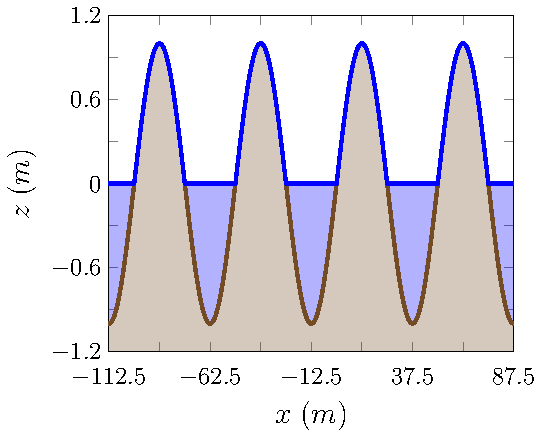
\includegraphics[width=\textwidth]{./chp5/figures/Analytic/LakeAtRest/Example/FEVMWB.pdf}
		\subcaption{$\text{FEVM}_2$ well-balanced}
		\vspace{0.5cm}
	\end{subfigure}%
	\begin{subfigure}{0.5\textwidth}
		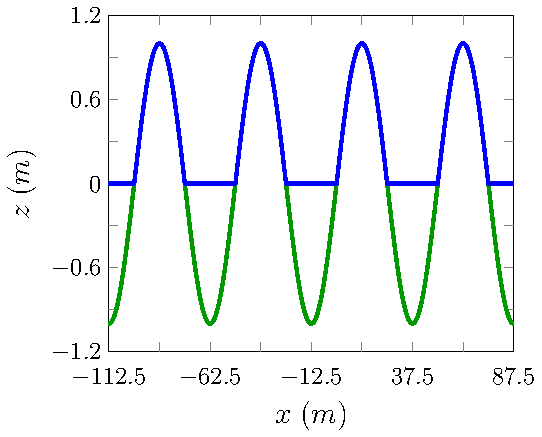
\includegraphics[width=\textwidth]{./chp5/figures/Analytic/LakeAtRest/Example/FEVMnWB.pdf}
		\subcaption{$\text{FEVM}_2$ not well-balanced}
		\vspace{0.5cm}
	\end{subfigure}
	\begin{subfigure}{0.5\textwidth}
		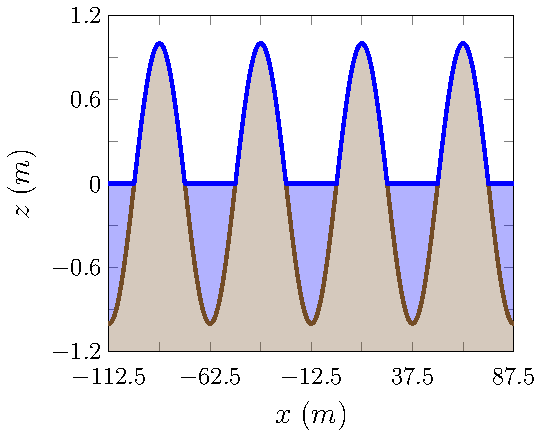
\includegraphics[width=\textwidth]{./chp5/figures/Analytic/LakeAtRest/Example/FDVMWB.pdf}
		\subcaption{$\text{FDVM}_2$ well-balanced}
	\end{subfigure}%
	\begin{subfigure}{0.5\textwidth}
		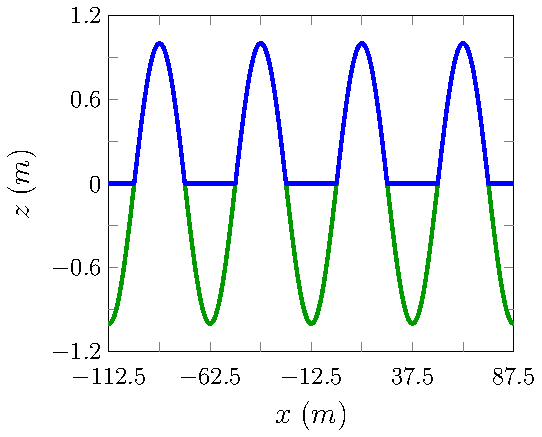
\includegraphics[width=\textwidth]{./chp5/figures/Analytic/LakeAtRest/Example/FDVMnWB.pdf}
		\subcaption{$\text{FDVM}_2$ not well-balanced}
	\end{subfigure}
	\caption{Numerical solutions for $w$ (\squareF{blue}) and $b$ (\squareF{brown!60!black}) with $\Delta x = {100} / {2^{10}}m $ for the lake at rest problem at $t=10s$ for $\text{FEVM}_2$ and $\text{FDVM}_2$.}
	\label{fig:LakeAtRestEx}
\end{figure}

Examination of the $L_2$ errors depicted in Figure \ref{fig:LakeAtRestEL1} reveals that only the well-balanced methods have accurately recovered the analytic solution. With both well-balanced versions of the methods reproducing $h$, $G$ and $u$ precisely, accounting for round-off errors. For $G$ and $u$ their errors are increasing due to an accumulation of the round-off errors for each cell and time step; hence their second-order increase as $\Delta x \rightarrow 0$. The errors in $u$ produce errors in $h$ through its flux function increasing the error in $h$ as $\Delta x$ decreases. However, since $h$ is far larger than $u$ these effects have a more complicated relationship to the cell width.

\begin{figure}
	\centering
	\begin{subfigure}{0.5\textwidth}
		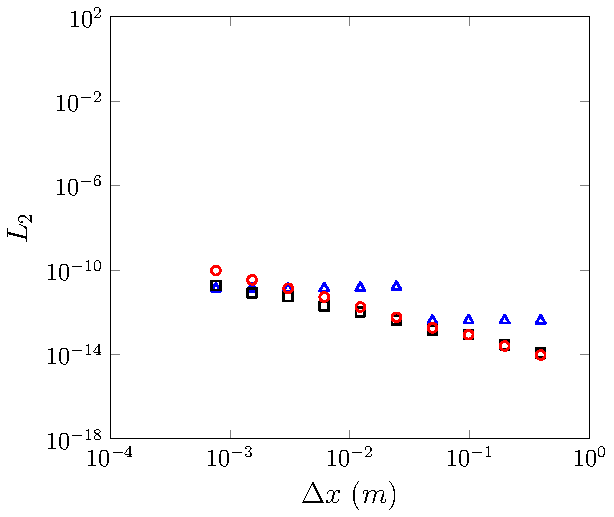
\includegraphics[width=\textwidth]{./chp5/figures/Analytic/LakeAtRest/L2/FEVMWB.pdf}
		\subcaption{$\text{FEVM}_2$ well-balanced}
		\vspace{0.3cm}
	\end{subfigure}%
	\begin{subfigure}{0.5\textwidth}
		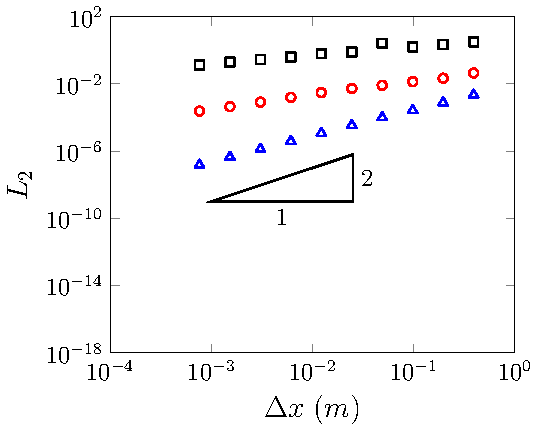
\includegraphics[width=\textwidth]{./chp5/figures/Analytic/LakeAtRest/L2/FEVMnWB.pdf}
		\subcaption{$\text{FEVM}_2$ not well-balanced}
		\vspace{0.3cm}
	\end{subfigure}
	\begin{subfigure}{0.5\textwidth}
		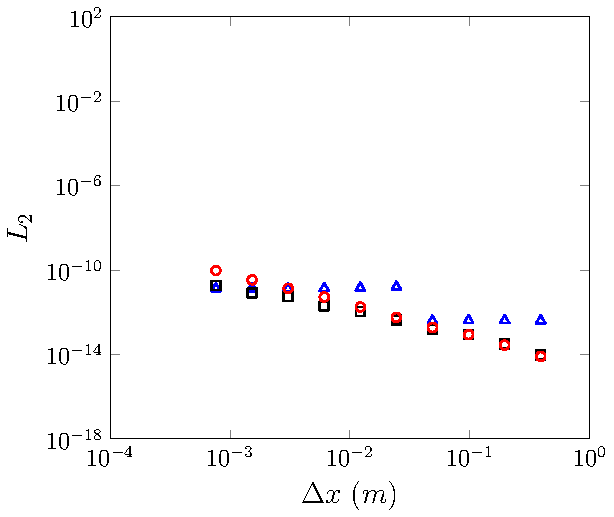
\includegraphics[width=\textwidth]{./chp5/figures/Analytic/LakeAtRest/L2/FDVMWB.pdf}
		\subcaption{$\text{FDVM}_2$ well-balanced}
	\end{subfigure}%
	\begin{subfigure}{0.5\textwidth}
		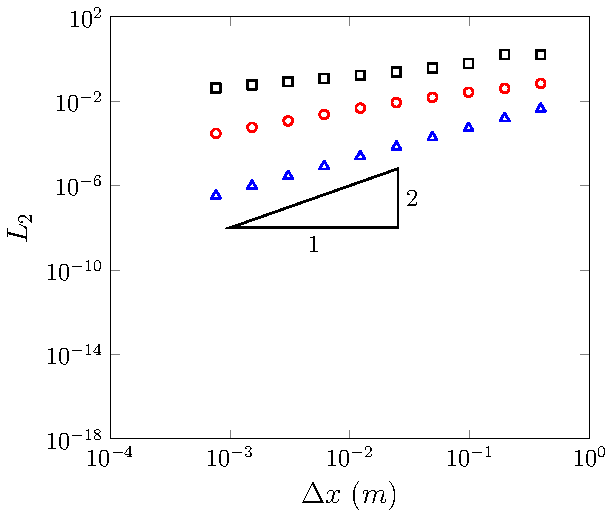
\includegraphics[width=\textwidth]{./chp5/figures/Analytic/LakeAtRest/L2/FDVMnWB.pdf}
		\subcaption{$\text{FDVM}_2$ not well-balanced}
	\end{subfigure}
	\caption{Convergence as measured by the $L_2$ norm against $\Delta x$ for $h$ (\trianglet{blue}), $u$ (\squaret{black}) and $G$ (\circlet{red}) for the lake at rest problem at $t=10s$ $\text{FEVM}_2$ and $\text{FDVM}_2$.}
	\label{fig:LakeAtRestEL1}
\end{figure}

For methods without well-balancing; the errors are significantly larger, yet they are converging to the analytic solution. However, the order of accuracy of the convergence in $u$ and $G$ has degraded and is not the expected second-order accuracy observed for $h$. The poor convergence of $u$ and $G$ is a result of the errors in $u$ and $G$ not being damped by the method. Thus errors generated by the imbalance between the flux and source terms increase over time degrading the order of accuracy. The second-order accuracy in $h$ is retained for the presented $\Delta x$ values as these errors introduced in $u$ and $G$ are small for a single cell, although for smaller $\Delta x$ values these errors in $u$ and $G$ will begin to dominate the errors in $h$. 


%%%%%%[][][][] NEW [][][][][]
Using the expressions in Appendix \ref{app:ConQuant} for the total amounts of the conserved quantities the conservation error $C$ was calculated for $\text{FEVM}_2$ and $\text{FDVM}_2$ with the results plotted in Figure \ref{fig:LakeAtRestEC1}. The error in conservation of these methods affirms the superiority of the well-balanced version of the methods. In particular, we see that the total amounts of $uh$ and $G$ are only conserved within machine precision when well-balancing is employed. Since $uh$ and $G$ are uniformly zero in the initial conditions the well-balanced methods have only introduced round-off errors into these quantities, whilst without well-balancing large errors in these quantities are introduced in the naive methods. 

The errors in conservation of $h$ and $\mathcal{H}$ for the well-balanced methods are large, but do converge at the order of accuracy of the scheme or better. These errors are caused by the discretisation of the initial conditions, primarily the approximation of the boundaries of the wet regions by the numerical grids. This initial discretisation error can be removed by comparing the total amounts of the conserved quantities in the numerical solution to their numerically calculated total amounts in the initial conditions with $C^*$ as in Figure \ref{fig:LakeAtRestEC*1}. For the completely numerically calculated conservation error $C^*$ we observe that all the conserved quantities are conserved at machine precision for the well-balanced methods. With $\mathcal{H}$ being conserved exactly for most numerical solutions, hence its disappearance from the log-log plot. The conservation error of $\mathcal{H}$ is small for the lake at rest solution since $u$ is very small. Hence, $\mathcal{H}$ is essentially the gravitational potential energy which since mass is well conserved is also well conserved.

%mention hamilton
\begin{figure}
	\centering
	\begin{subfigure}{0.5\textwidth}
		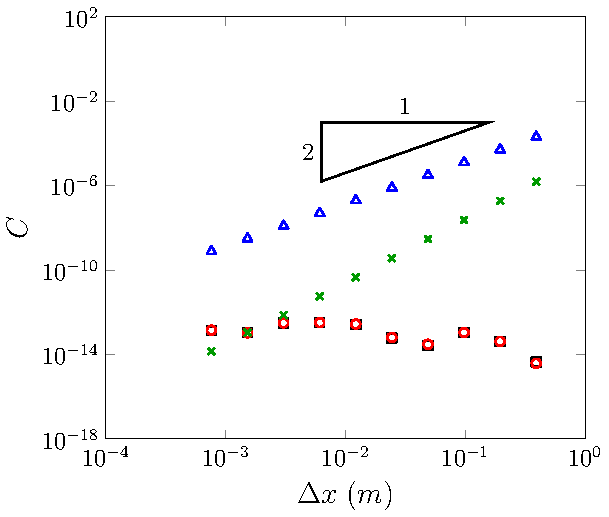
\includegraphics[width=\textwidth]{./chp5/figures/Analytic/LakeAtRest/C1/Ana/FEVM2WB.pdf}
		\subcaption{$\text{FEVM}_2$ well-balanced}
		\vspace{0.5cm}
	\end{subfigure}%
	\begin{subfigure}{0.5\textwidth}
		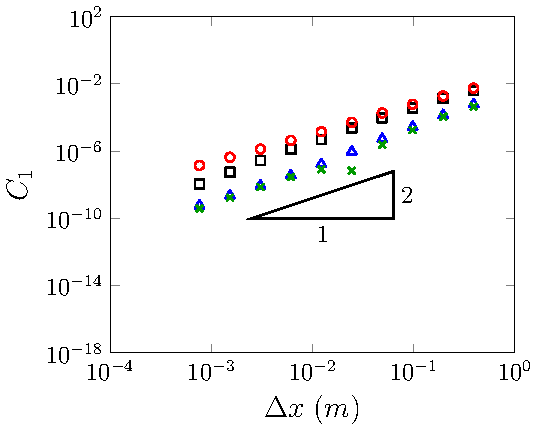
\includegraphics[width=\textwidth]{./chp5/figures/Analytic/LakeAtRest/C1/Ana/FEVM2nWB.pdf}
		\subcaption{$\text{FEVM}_2$ not well-balanced}
		\vspace{0.5cm}
	\end{subfigure}
	\begin{subfigure}{0.5\textwidth}
		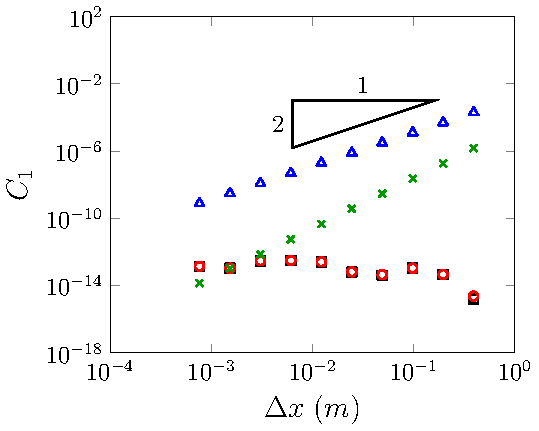
\includegraphics[width=\textwidth]{./chp5/figures/Analytic/LakeAtRest/C1/Ana/FDVM2WB.pdf}
		\subcaption{$\text{FDVM}_2$ well-balanced}
	\end{subfigure}%
	\begin{subfigure}{0.5\textwidth}
		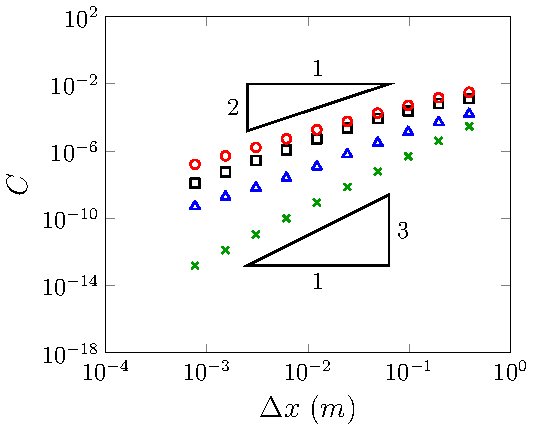
\includegraphics[width=\textwidth]{./chp5/figures/Analytic/LakeAtRest/C1/Ana/FDVM2nWB.pdf}
		\subcaption{$\text{FDVM}_2$ not well-balanced}
	\end{subfigure}
	\caption{Conservation error $C$ against $\Delta x$ for $h$ (\trianglet{blue}), $uh$ (\squaret{black}), $G$ (\circlet{red}) and $\mathcal{H}$ ({\color{green!60!black} \crosst{green!60!black}}) for the lake at rest problem at $t=10s$ for $\text{FEVM}_2$ and $\text{FDVM}_2$.}
	\label{fig:LakeAtRestEC1}
\end{figure}

\begin{figure}
	\centering
	\begin{subfigure}{0.5\textwidth}
		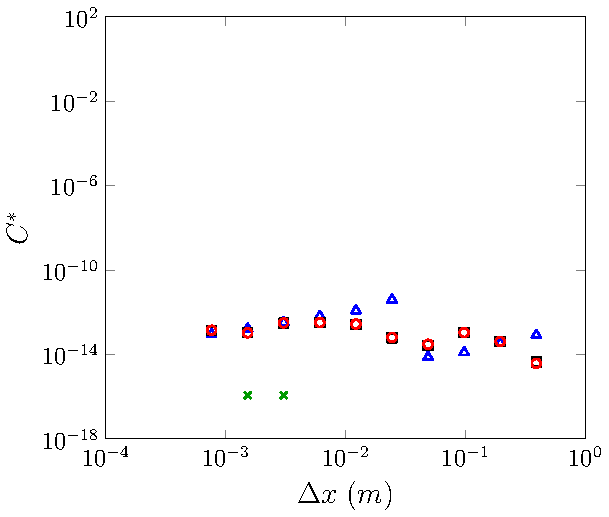
\includegraphics[width=\textwidth]{./chp5/figures/Analytic/LakeAtRest/C1/Num/FEVM2WB.pdf}
		\subcaption{$\text{FEVM}_2$ well-balanced}
		\vspace{0.5cm}
	\end{subfigure}%
	\begin{subfigure}{0.5\textwidth}
		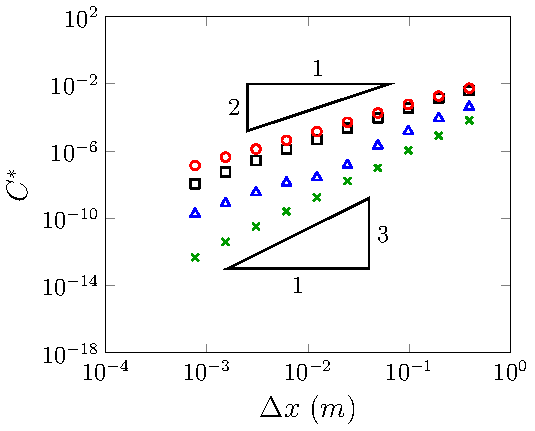
\includegraphics[width=\textwidth]{./chp5/figures/Analytic/LakeAtRest/C1/Num/FEVM2nWB.pdf}
		\subcaption{$\text{FEVM}_2$ not well-balanced}
		\vspace{0.5cm}
	\end{subfigure}
	\begin{subfigure}{0.5\textwidth}
		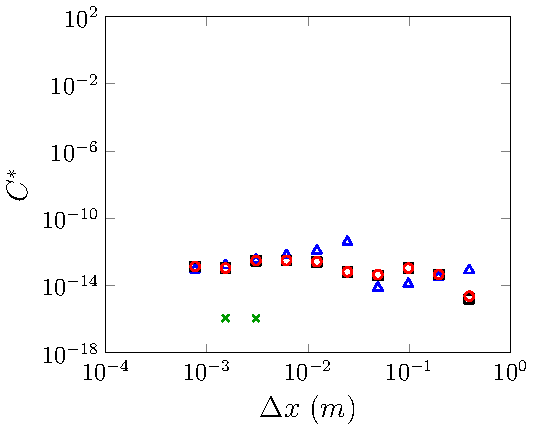
\includegraphics[width=\textwidth]{./chp5/figures/Analytic/LakeAtRest/C1/Num/FDVM2WB.pdf}
		\subcaption{$\text{FDVM}_2$ well-balanced}
	\end{subfigure}%
	\begin{subfigure}{0.5\textwidth}
		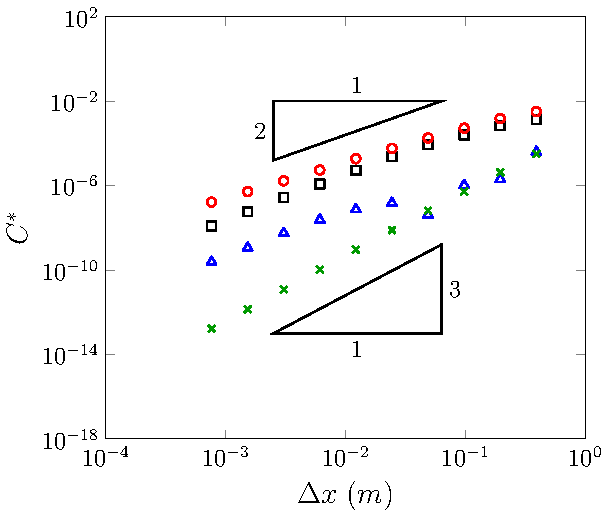
\includegraphics[width=\textwidth]{./chp5/figures/Analytic/LakeAtRest/C1/Num/FDVM2nWB.pdf}
		\subcaption{$\text{FDVM}_2$ not well-balanced}
	\end{subfigure}
	\caption{Conservation error using only numerical calculations $C^*$ against $\Delta x$ for $h$ (\trianglet{blue}), $uh$ (\squaret{black}), $G$ (\circlet{red}) and $\mathcal{H}$ ({\color{green!60!black} \crosst{green!60!black}}) for the lake at rest problem at $t=10s$ for $\text{FEVM}_2$ and $\text{FDVM}_2$.}
	\label{fig:LakeAtRestEC*1}
\end{figure}   

These results demonstrate the need for well-balancing for both numerical methods, as it is only with its inclusion that the lake at rest steady state can be accurately reproduced. 


\section{Forced Solutions}
%only L1
The previous analytic solution validations do not provide a stringent test for all terms present in the Serre equations and there are currently no known analytic solutions that do. To remedy this the forced solutions introduced in Chapter \ref{chp:Serreeqns} were used to validate the numerical methods. Since the source terms in the modified Serre equations, \eqref{eqn:FullSerreConForced} can be determined and accounted for analytically, the only source of error in the numerical solutions reproduction of the forced solutions are the numerical methods themselves and thus the theoretical second-order accuracy of $\text{FEVM}_2$ and $\text{FDVM}_2$ should be recovered. 

We performed validation tests for two forced solutions; one with a finite water depth everywhere and the other with a dry bed to validate and compare the numerical solutions in both situations. To ensure that all terms of the Serre equations were accurately approximated in the numerical method the functions
\begin{subequations}
\begin{align}
\label{eqn:ForcedSolutionxt}
h^*(x,t) &= a_0 + a_1 \exp\left(-\dfrac{\left[\left(x - a_2 t\right) - a_3\right]^2}{2 a_4}\right), \\
u^*(x,t) &= a_5 \exp\left(-\dfrac{\left[\left(x - a_2 t\right) - a_3\right]^2}{2 a_4}\right), \\
b^*(x) &= a_6 \sin\left(a_7 x\right)
\end{align}
\end{subequations}
for the primitive variables were chosen. These functions produce an $a_1$ high Gaussian bump for $h$ and $u$ that travels at a fixed speed $a_2$ over a periodic bed. Thus, $h$ and $u$ will have constant shape and travel to the right over time. However, this is not the case for $G$ as $u$ and $h$ have constant shape but the bed is periodic. With the bed terms in $G$ \eqref{defn:SerreEqnConservedQuantity1} changing the shape of $G$ as the Gaussian bump in $h$ and $u$ encounters different bed slopes.

For non-trivial choices of the parameters $a_i$ all terms in the Serre equations vary in space and time and so all terms must be accurately approximated by the numerical method to adequately reproduce the forced solution. 

Both validation studies used the values $a_1 = 0.5m$, $a_2 = 2 \pi / \left(10 a_7\right) m/s$, $a_3 =- 3\pi/ \left(2 a_7\right)m$, $a_4 = \pi / (16 a_7) m^2$, $a_5 = 0.5 m/s$, $a_6 = 1.0 m$ and $a_7 = \pi / 25 m^{-1}$ with $a_0= 1m$ for the finite water depth forced solution and $a_0=0m$ for the dry bed forced solution. These parameter values result in a Gaussian bump in $h$ and $u$ that has a width much smaller than the wavelength of the bed profile and travels precisely one wavelength in $10s$.

The domain of the numerical solutions was $x \in \left[-112.5 m,87.5 m\right]$ with $t \in \left[0s,10s\right]$. The standard gravitational acceleration $g= 9.81 m/s^2$ was used. The spatial resolution of numerical methods was varied like so $\Delta x = 100 / 2^k m$ with $k \in \left[8,\dots,17\right]$. To satisfy the CFL condition, \eqref{eqn:CFLcond} the temporal resolution
$\Delta t = Cr \Delta x / \left(a_2 + a_5 + \sqrt{g\left(a_0 + a_1\right)}\right)$ was chosen with condition number $Cr = 0.5$. The value $\theta = 1.2$ was used in the generalised minmod limiter \eqref{eqn:slopehGrecon} for both $\text{FEVM}_2$ and $\text{FDVM}_2$ and Dirichlet boundary conditions were applied at the boundaries of the domain. 


\subsection{Results for a Wet Bed} 
%a_0 = 1
For the non-zero water depth case where $a_0 = 1m$ an example of the numerical solutions of $\text{FEVM}_2$ and $\text{FDVM}_2$ are given in Figures \ref{fig:ForcedWetFEVMP2PExAll} and \ref{fig:ForcedWetFDVMP2PExAll} respectively for $\Delta x = 100/ 2^{10} m \approx 0.0977m $ at various times. The numerical solutions and the forced solutions are indistinguishable at all times for these scales, accurately reproducing the forced solution as it travels over the bed. Thus $h$ and $u$ maintain their constant shape while $G$ does not due to the influence of the periodic bed.
\begin{figure}
	\centering
	\begin{subfigure}{0.5\textwidth}
		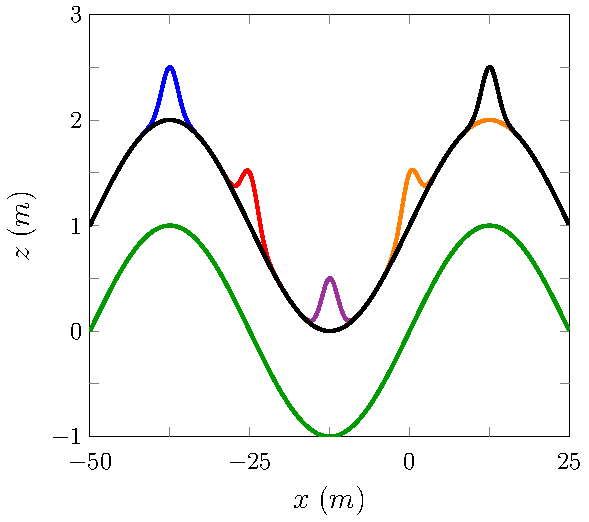
\includegraphics[width=\textwidth]{./chp5/figures/Forced/Wet/FEVMw.pdf}
		\subcaption{$w$ and $b$ (\squareF{brown!60!black})}
		\vspace{0.5cm}
	\end{subfigure}%
	\begin{subfigure}{0.5\textwidth}
		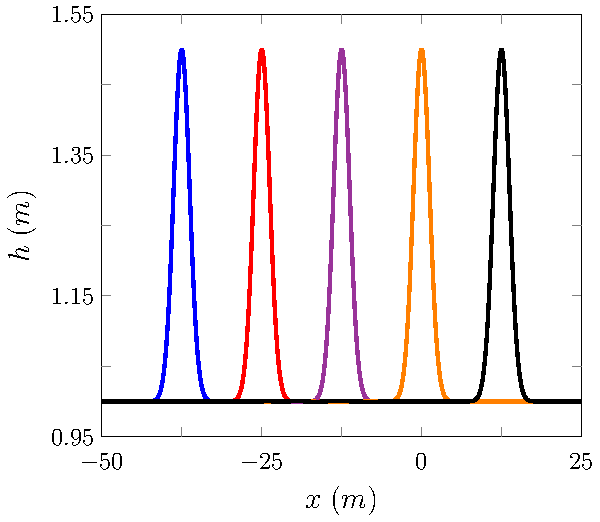
\includegraphics[width=\textwidth]{./chp5/figures/Forced/Wet/FEVMh.pdf}
		\subcaption{$h$}
		\vspace{0.5cm}
	\end{subfigure}
	\begin{subfigure}{0.5\textwidth}
		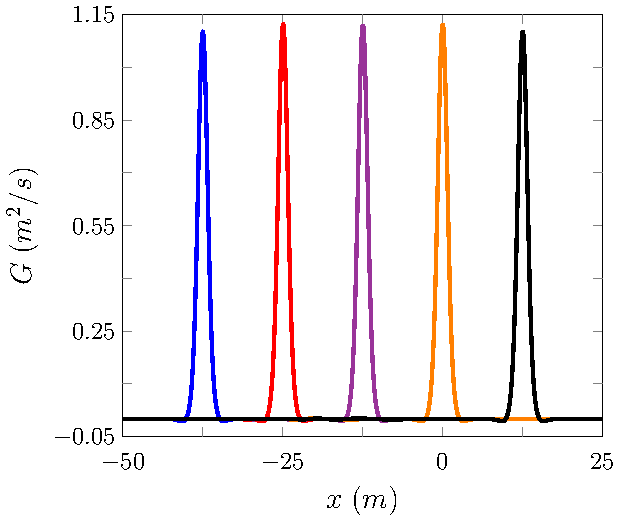
\includegraphics[width=\textwidth]{./chp5/figures/Forced/Wet/FEVMG.pdf}
		\subcaption{$G$}
	\end{subfigure}%
	\begin{subfigure}{0.5\textwidth}
		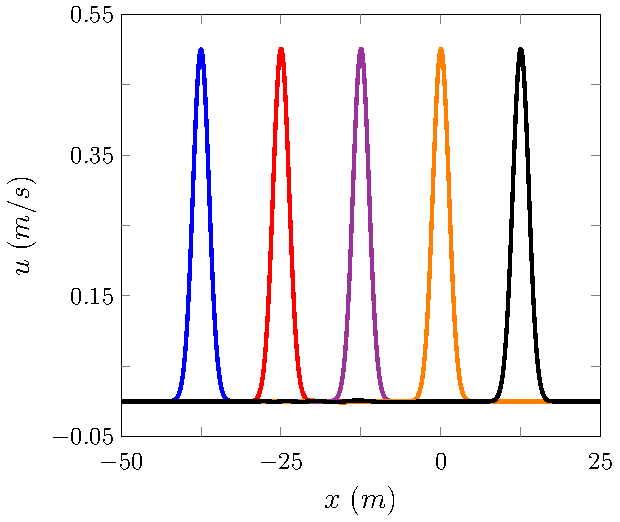
\includegraphics[width=\textwidth]{./chp5/figures/Forced/Wet/FEVMu.pdf}
		\subcaption{$u$}
	\end{subfigure}
	\caption{Numerical solutions for $w$, $b$, $h$, $G$ and $u$ produced by $\text{FEVM}_2$ with $\Delta x = 100 / 2^{10}m$ at $t=$ $0s$ ({\color{blue} \solidrule} / \squareF{blue} ), $2.5s$ ({\color{red} \solidrule}/ \squareF{red}), $5.0s$ ({\color{violet!80!white} \solidrule} / \squareF{violet!80!white}), $7.5s$ ({\color{orange} \solidrule}/ \squareF{orange}), $10.0s$ ({\color{black} \solidrule} / \squareF{black}) to the wet bed forced solution problem, where $a_0 = 1m$.}
	\label{fig:ForcedWetFEVMP2PExAll}
\end{figure}
\begin{figure}
	\centering
	\begin{subfigure}{0.5\textwidth}
		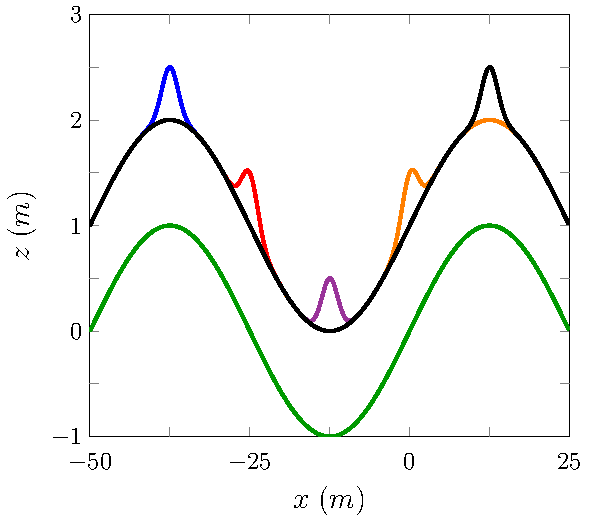
\includegraphics[width=\textwidth]{./chp5/figures/Forced/Wet/FDVMw.pdf}
		\subcaption{$w$ and $b$ (\squareF{brown!60!black})}
		\vspace{0.5cm}
	\end{subfigure}%
	\begin{subfigure}{0.5\textwidth}
		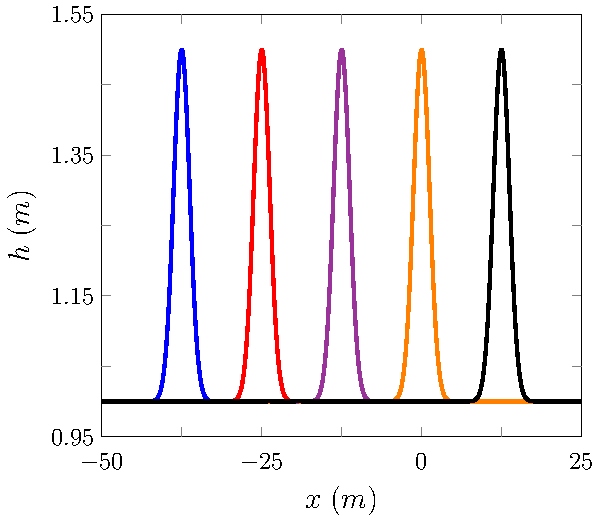
\includegraphics[width=\textwidth]{./chp5/figures/Forced/Wet/FDVMh.pdf}
		\subcaption{$h$}
		\vspace{0.5cm}
	\end{subfigure}
	\begin{subfigure}{0.5\textwidth}
		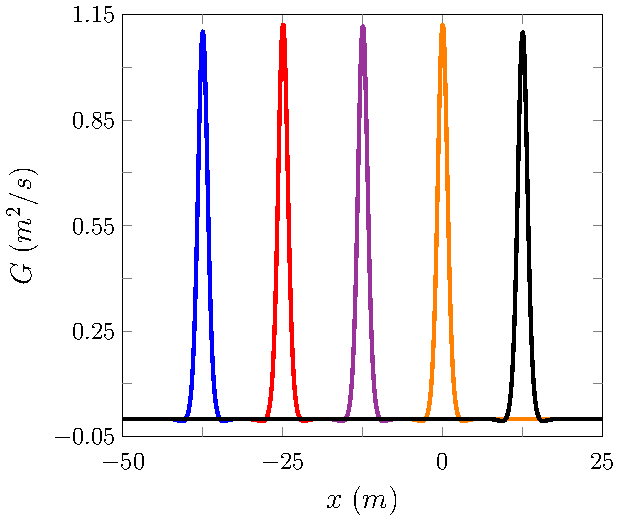
\includegraphics[width=\textwidth]{./chp5/figures/Forced/Wet/FDVMG.pdf}
		\subcaption{$G$}
	\end{subfigure}%
	\begin{subfigure}{0.5\textwidth}
		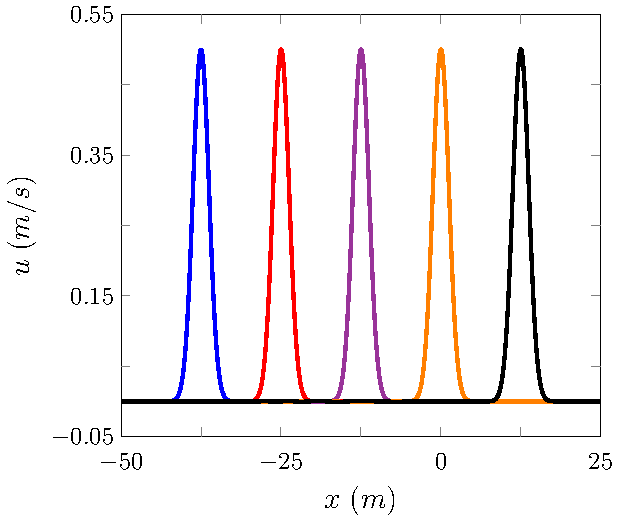
\includegraphics[width=\textwidth]{./chp5/figures/Forced/Wet/FDVMu.pdf}
		\subcaption{$u$}
	\end{subfigure}
	\caption{Numerical solutions for $w$, $b$, $h$, $G$ and $u$ produced by $\text{FDVM}_2$ with $\Delta x = 100 / 2^{10}m$ at $t=$ $0s$ ({\color{blue} \solidrule} / \squareF{blue} ), $2.5s$ ({\color{red} \solidrule}/ \squareF{red}), $5.0s$ ({\color{violet!80!white} \solidrule} / \squareF{violet!80!white}), $7.5s$ ({\color{orange} \solidrule}/ \squareF{orange}), $10.0s$ ({\color{black} \solidrule} / \squareF{black}) to the wet bed forced solution problem, where $a_0 = 1m$.}
	\label{fig:ForcedWetFDVMP2PExAll}
\end{figure}

The $L_2$ error of $h$, $u$ and $G$ for the $\text{FEVM}_2$ and $\text{FDVM}_2$ are given in Figure \ref{fig:L1convergenceforcedWet}. Both methods recover the expected second-order accuracy. Since the term of the forced Serre equations is added analytically and all terms must be accurately approximated by the method for this forced solution, these results demonstrate that $\text{FEVM}_2$ and $\text{FDVM}_2$ are second-order accurate for all terms when the bed is wet everywhere, as desired.

\begin{figure}
	\centering
	\begin{subfigure}{0.5\textwidth}
		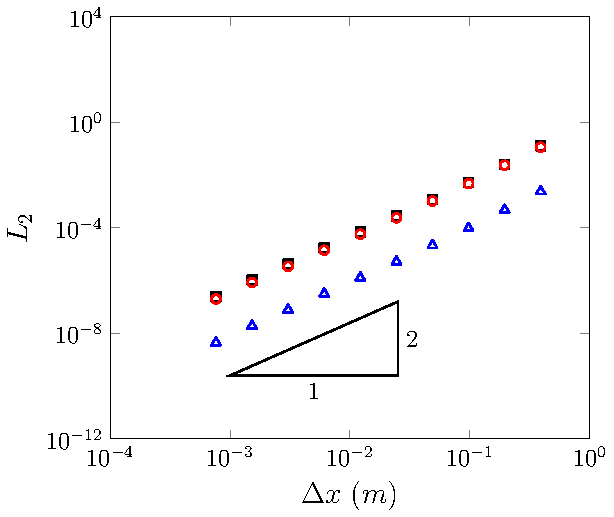
\includegraphics[width=\textwidth]{./chp5/figures/Forced/Wet/FEVML2.pdf}
		\subcaption{$\text{FEVM}_2$}
	\end{subfigure}%
	%[]!!---!![]
	\begin{subfigure}{0.5\textwidth}
		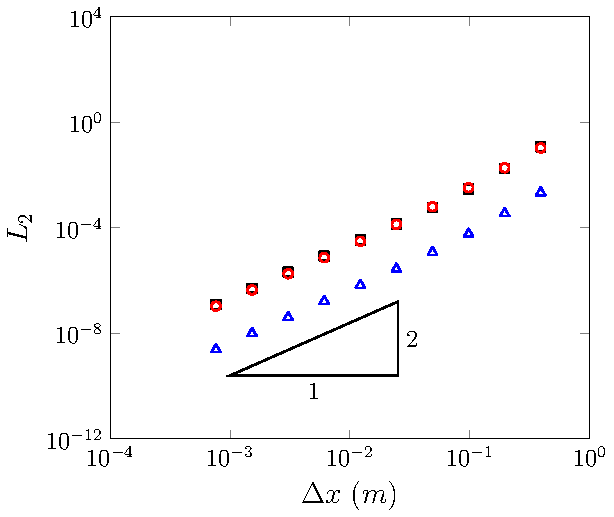
\includegraphics[width=\textwidth]{./chp5/figures/Forced/Wet/FDVML2.pdf}
		\subcaption{$\text{FDVM}_2$}
	\end{subfigure}
	\caption{Convergence as measured by the $L_2$ norm against $\Delta x$ for $h$ (\trianglet{blue}), $u$ (\squaret{black}) and $G$ (\circlet{red}) for the wet bed forced solution problem for $\text{FEVM}_2$ and $\text{FDVM}_2$ at $t=10s$.}
	\label{fig:L1convergenceforcedWet}
\end{figure}


\subsection{Results with a Dry Bed} 
%a_0 = 0
%mention the tolerance values
To demonstrate the capability of the methods to handle wetting and drying of a bed, a series of numerical simulations of the forced solutions \eqref{eqn:ForcedSolutionxt} where $a_0 = 0m$ were conducted using both $\text{FEVM}_2$ and $\text{FDVM}_2$. 

Example numerical solutions demonstrating the evolution of the wave are given in Figure \ref{fig:ForcedFEVMP2PExAll} for $\text{FEVM}_2$ and Figure \ref{fig:ForcedFDVMP2PExAll} $\text{FDVM}_2$ with $\Delta x = 100/ 2^{10} m \approx 0.0977m$ at various times. The methods accurately reproduce the analytic solution for the stage $w$, $h$ and $G$. However, both fail to accurately reproduce $u$ when $h$ is small, particularly behind the Gaussian bump. So that now $h$ is the only quantity that maintains a constant shape in the numerical solutions, as $G$ changes due to the periodic bed and $u$ changes due to numerical errors. 

\begin{figure}
	\centering
	\begin{subfigure}{0.5\textwidth}
		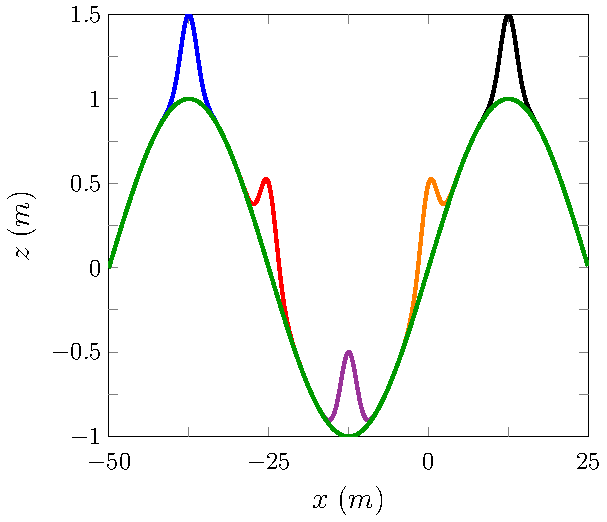
\includegraphics[width=\textwidth]{./chp5/figures/Forced/Dry/FEVMw.pdf}
		\subcaption{$w$ and $b$ (\squareF{brown!60!black})}
		\vspace{0.5cm}
	\end{subfigure}%
	\begin{subfigure}{0.5\textwidth}
		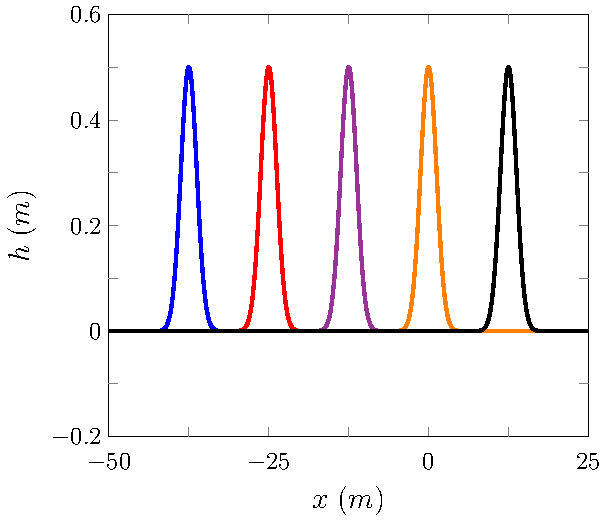
\includegraphics[width=\textwidth]{./chp5/figures/Forced/Dry/FEVMh.pdf}
		\subcaption{$h$}
		\vspace{0.5cm}
	\end{subfigure}
	\begin{subfigure}{0.5\textwidth}
		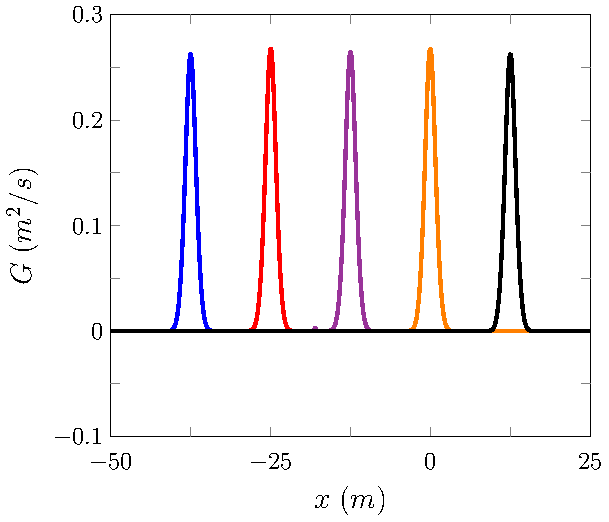
\includegraphics[width=\textwidth]{./chp5/figures/Forced/Dry/FEVMG.pdf}
		\subcaption{$G$}
	\end{subfigure}%
	\begin{subfigure}{0.5\textwidth}
		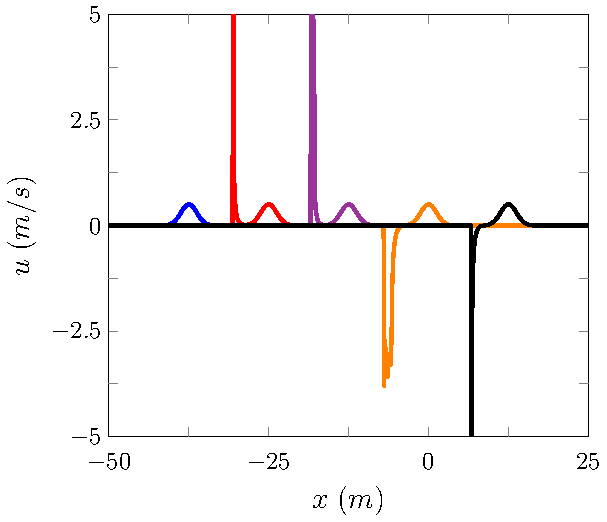
\includegraphics[width=\textwidth]{./chp5/figures/Forced/Dry/FEVMu.pdf}
		\subcaption{$u$}
	\end{subfigure}
	\caption{Numerical solutions for $w$, $b$, $h$, $G$ and $u$ produced by $\text{FEVM}_2$ with $\Delta x = 100 / 2^{10}m$ at $t=$ $0s$ ({\color{blue} \solidrule} / \squareF{blue} ), $2.5s$ ({\color{red} \solidrule}/ \squareF{red}), $5.0s$ ({\color{violet!80!white} \solidrule} / \squareF{violet!80!white}), $7.5s$ ({\color{orange} \solidrule}/ \squareF{orange}), $10.0s$ ({\color{black} \solidrule} / \squareF{black}) to the dry bed forced solution problem, where $a_0 = 0m$.}
	\label{fig:ForcedFEVMP2PExAll}
\end{figure}
\begin{figure}
	\centering
	\begin{subfigure}{0.5\textwidth}
		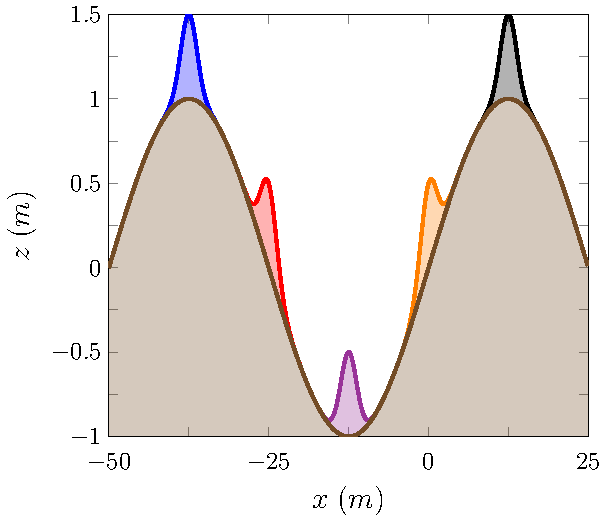
\includegraphics[width=\textwidth]{./chp5/figures/Forced/Dry/FDVMw.pdf}
		\subcaption{$w$ and $b$ (\squareF{brown!60!black})}
		\vspace{0.5cm}
	\end{subfigure}%
	\begin{subfigure}{0.5\textwidth}
		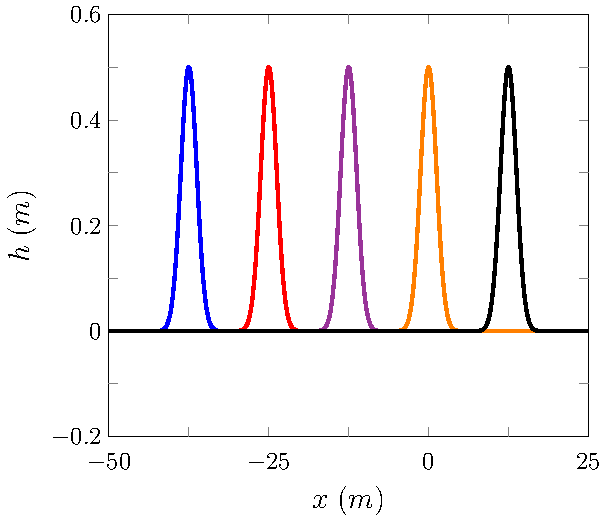
\includegraphics[width=\textwidth]{./chp5/figures/Forced/Dry/FDVMh.pdf}
		\subcaption{$h$}
		\vspace{0.5cm}
	\end{subfigure}
	\begin{subfigure}{0.5\textwidth}
		\includegraphics[width=\textwidth]{./chp5/figures/Forced/Dry/FDVMG.pdf}
		\subcaption{$G$}
	\end{subfigure}%
	\begin{subfigure}{0.5\textwidth}
		\includegraphics[width=\textwidth]{./chp5/figures/Forced/Dry/FDVMu.pdf}
		\subcaption{$u$}
	\end{subfigure}
	\caption{Numerical solutions for $w$, $b$, $h$, $G$ and $u$ produced by $\text{FDVM}_2$ with $\Delta x = 100 / 2^{10}m$ at $t=$ $0s$ ({\color{blue} \solidrule} / \squareF{blue} ), $2.5s$ ({\color{red} \solidrule}/ \squareF{red}), $5.0s$ ({\color{violet!80!white} \solidrule} / \squareF{violet!80!white}), $7.5s$ ({\color{orange} \solidrule}/ \squareF{orange}), $10.0s$ ({\color{black} \solidrule} / \squareF{black}) to the dry bed forced solution problem, where $a_0 = 0m$.}
	\label{fig:ForcedFDVMP2PExAll}
\end{figure}

These large errors in $u$ when $h$ is small are caused by the particular choices $h_{{base}} = 10^{-8}$ and $h_{{tol}}  = 10^{-12}$ used in the desingularisation transformation applied to the FEM \eqref{eqn:usolvefromGhb}. By choosing larger values of these quantities the errors in $u$ can be significantly damped. However, if $h_{{base}}$ and $h_{{tol}}$ are larger they begin to dominate the $L_2$ errors in $h$, $G$ and $uh$ making the convergence less obvious. This trade-off is present in all desingularisation transforms. 

For our purposes the chosen desingularisation transform \eqref{eqn:hdrytransform} with small $h_{{base}}$ and $h_{{tol}}$ values was sufficient, resulting in large observed errors in $u$ when $h$ is small.


%%%%% [][][] NEW [][][]
The $L_2$ errors for $h$, $u$, $uh$ and $G$ for both methods are given in Figure \ref{fig:ForcedSolDryL1}. Both methods exhibit second-order convergence in all the quantities except $u$. The large errors in $u$ only occur when $h$ is small. This can be seen by restricting our convergence to only compare regions where $h > 10^{-3} m$ as in Figure \ref{fig:ForcedSolDryL1restrict}. It can be seen that the expected second-order accuracy in $u$ is recovered when $h$ is not small. Since all the flux and source terms of the Serre equations \eqref{eqn:FullSerreCon} only depend on $u$ multiplied by some power of $h$; the large errors in $u$ when $h$ is small do not translate to significant errors in $G$, $h$ or $uh$. 

Therefore, these methods can accurately handle the dry bed problem, even with small $h_{{base}}$ and $h_{{tol}}$ values, although in such cases the velocity may have large errors in regions where $h$ is small. For physical applications where large errors in $u$ when $h$ is small are not acceptable we recommend altering the dry bed handling of the scheme by increasing the $h_{{base}}$ and $h_{{tol}}$ values or altering the desingularisation transformation \cite{Kurganov-Petrova-2007-707}. 

\begin{figure}
	\centering
	\begin{subfigure}{0.5\textwidth}
		\includegraphics[width=\textwidth]{./chp5/figures/Forced/Dry/FEVML2.pdf}
		\subcaption{$\text{FEVM}_2$}
	\end{subfigure}%
	\begin{subfigure}{0.5\textwidth}
		\includegraphics[width=\textwidth]{./chp5/figures/Forced/Dry/FDVML2.pdf}
		\subcaption{$\text{FDVM}_2$}
	\end{subfigure}
	\caption{Convergence as measured by the $L_2$ norm against $\Delta x$ for $h$ (\trianglet{blue}), $u$ (\squaret{black}), $uh$ ({\crosst{green!60!black}}) and $G$ (\circlet{red}) for the dry bed forced solution problem for $\text{FEVM}_2$ and $\text{FDVM}_2$ at $t=10s$.}
	\label{fig:ForcedSolDryL1}
\end{figure}

\begin{figure}
	\centering
	\begin{subfigure}{0.5\textwidth}
		\includegraphics[width=\textwidth]{./chp5/figures/Forced/Dry/FEVML2red.pdf}
		\subcaption{$\text{FEVM}_2$}
		\vspace{0.5cm}
	\end{subfigure}%
	%[]!!---!![]
	\begin{subfigure}{0.5\textwidth}
		\includegraphics[width=\textwidth]{./chp5/figures/Forced/Dry/FDVML2red.pdf}
		\subcaption{$\text{FDVM}_2$}
		\vspace{0.5cm}
	\end{subfigure}
	\caption{Convergence for regions where $h > 10^{-3}m$ as measured by the $L_2$ norm against $\Delta x$ for $h$ (\trianglet{blue}), $u$ (\squaret{black}) and $G$ (\circlet{red}) for the dry bed forced solution problem for $\text{FEVM}_2$ and $\text{FDVM}_2$ at $t=10s$.}
	\label{fig:ForcedSolDryL1restrict}
\end{figure}

\medskip
In this chapter the analytic and forced solutions were used to assess the numerical methods. It was found that the finite volume based methods performed better than the finite difference methods and that second-order methods were sufficient to accurately reproduce the analytic solutions. Finally the second-order accuracy of $\text{FEVM}_2$ and $\text{FDVM}_2$ was confirmed for the wetting and drying of variable beds using forced solutions to the Serre equations.
